%%%%%%%%%%%%%%%%%%%%%%% file typeinst.tex %%%%%%%%%%%%%%%%%%%%%%%%%
%
% This is the LaTeX source for the instructions to authors using
% the LaTeX document class 'llncs.cls' for contributions to
% the Lecture Notes in Computer Sciences series.
% http://www.springer.com/lncs       Springer Heidelberg 2006/05/04
%
% It may be used as a template for your own input - copy it
% to a new file with a new name and use it as the basis
% for your article.
%
% NB: the document class 'llncs' has its own and detailed documentation, see
% ftp://ftp.springer.de/data/pubftp/pub/tex/latex/llncs/latex2e/llncsdoc.pdf
%
%%%%%%%%%%%%%%%%%%%%%%%%%%%%%%%%%%%%%%%%%%%%%%%%%%%%%%%%%%%%%%%%%%%

\documentclass[runningheads,a4paper,10pt]{llncs}

\usepackage[utf8]{inputenc}
\usepackage[left=3cm,right=3cm,top=3cm,bottom=3cm]{geometry}

\usepackage{natbib}
\bibliographystyle{apalike-fr}

\usepackage{amssymb}
\setcounter{tocdepth}{3}
\usepackage{graphicx}

\usepackage[hidelinks]{hyperref}

\usepackage{caption}

\usepackage{amsmath}

\usepackage[french]{babel} % Pour adopter les règles de typographie française
\usepackage[T1]{fontenc} % Pour que les lettres accentuées soient reconnues

\usepackage{url}
\urldef{\mailsa}\path|{alfred.hofmann, ursula.barth, ingrid.haas, frank.holzwarth,|
\urldef{\mailsb}\path|anna.kramer, leonie.kunz, christine.reiss, nicole.sator,|
\urldef{\mailsc}\path|erika.siebert-cole, peter.strasser, lncs}@springer.com|    
\newcommand{\keywords}[1]{\par\addvspace\baselineskip
\noindent\keywordname\enspace\ignorespaces#1}

\begin{document}

\mainmatter 

\title{Mini Mémoire \\ Le Model-Checking de CTL}

\titlerunning{Le Model-Checking de CTL}

\author{BUI QUANG PHUONG Linh -- 000427796 \\ Promoteur : Prof. GEERAERTS Gilles}

\institute{Université Libre de Bruxelles}

\authorrunning{BUI QUANG PHUONG Linh}

\toctitle{Abstract}
\tocauthor{{}}

\maketitle


\begin{abstract}
La vérification de modèles, plus communément appelée via son appellation anglaise \textit{Model-Checking}, est un système de vérification automatique qu'un système informatique ou électronique satisfasse une certaine propriété. Celle-ci est généralement utilisé afin de prouver la bonne fonctionnalité du système ou dans le cas contraire, de détecter des bugs ou des dysfonctionnements. Plusieurs types d'algorithmes et de logiques permettent d'effectuer un Model-Checking. Nous allons principalement nous intéresser au Model-Checking de CTL mis en place durant les années 80. 
\end{abstract}

\medskip

\begingroup
\let\clearpage\relax
\tableofcontents
\endgroup

\medskip
\medskip

\newpage 

\section{Introduction}

\subsection{Contexte et point de vue global}
\noindent
Les dernières décennies entrainant l'évolution exponentielle de la technologie et de l'informatique, la société actuelle fait régulièrement usage de systèmes automatisés afin d'assurer le bon fonctionnement et la fiabilité des programmes, machines et autres divers systèmes informatiques. Afin de vérifier ces systèmes, l'utilisation d'une technique algorithmique appelée \textit{Model-Checking} va être mise en place.  

\noindent
Le principe de base du model-checking est la vérification qu'un certain système satisfasse une certaine propriété. Le système sera représenté par un modèle $\mathcal{M}$ tandis que la propriété fera office d'une formule $\Phi$. Dans un premier temps, la modélisation du comportement dynamique du système est nécessaire avant d'être suivie par la vérification de la formule de la propriété grâce à l'algorithme de model-checking qui déterminera si le modèle satisfait bien la formule.  

$$\boxed{\mathcal{M} \vDash \Phi}$$

\noindent
Lorsque le système ne satisfait pas la propriété évaluée, le model-checking a donc repéré un bug ou un dysfonctionnement. Chaque année, le coût des bugs s'élève à environ 59 milliards de dollars \cite{ErrorCost} rien qu'aux Etats-Unis. La création et la mise en place de technique de vérification est donc impérative pour réduire le taux de bugs afin de minimiser ces coûts.  \\

\noindent
Illustrons cela par un exemple plus concret : un distributeur de boissons. Dans ce cas, il est indispensable que le montant demandé pour une certaine boisson soit mis dans la machine afin que le client puisse récupérer la boisson. La vérification de ce prérequis va être effectué à l'aide d'un système de model-checking. 
Un autre exemple illustrant l'importance du model-checking est la fermeture des barrières sur une voie ferrée lors du passage d'un train. 
Celle-ci doit être réalisée automatiquement lorsqu'un train est sur le point de traverser une voie ferrée. Dans ce cas, une petite erreur de timing peut avoir une très grande ampleur concernant la sécurité des passants. Il est donc impératif de vérifier la bonne fonctionnalité du système gérant la fermeture des barrières grâce au model-checking. 

\noindent 

\subsection{Les phases du model-checking}

Le processus de base d'un model-checking est divisé en 3 phases : 

\begin{enumerate}
 \item  \textbf{La phase de modélisation} : permet de représenter le comportement du système. Dans le cas du model-checking, cette phase de modélisation est réalisée à l'aide d'automates d'états finis\footnote{cfr. \autoref{sec:pdv-algo} "Point de vue algorithmique"} et de logique temporelle\footnote{cfr. \autoref{sec:log-temp} "Introduction à la logique temporelle"}. Celle-ci permet une formalisation du système ainsi que de la propriété à vérifier. De plus, cette modélisation permet de réaliser les premières vérifications grâce à différentes simulations réalisées sur le modèle. Cette phase de modélisation est l'objet de la \autoref{sec:pdv-algo} \textit{"Point de vue algorithmique"} et \autoref{sec:log-temp} \textit{"Introduction à la logique temporelle"}. 
 \item  \textbf{La phase d'exécution} : exécution du model-checker vérifiant la validité de la propriété à satisfaire. 
 \item  \textbf{La phase d'analyse} : lorsque les résultats sont obtenus après exécution, différents cas potentiels existent : 
 \begin{itemize}
 \item Si la propriété est \textbf{satisfaite} : vérification de la propriété suivante (si il y en a). 
 \item Si la propriété n'est \textbf{pas satisfaite} : soit un contre-exemple est produit qui décrit un scénario possible d’erreur (violation de la propriété), soit il y a correction du modèle et réexécution du model-checker, soit il y a réexécution de toute la procédure. 
 \item \textbf{Manque de mémoire} (cfr. \textit{State explosion problem}\footnote{\autoref{sec:desavantages} - 1er désavantage}): tentative de réduction du modèle notamment grâce aux diagrammes de décision binaire ou une réduction partielle de la commande et réexécution le model-checker. 
 \end{itemize}
 \end{enumerate} 
 
L'approche de model checking comprenant ses différents intérêts et différents phases est illustrée dans la \autoref{fig:schematic-view}.  
 
\begin{figure}
  \centering
   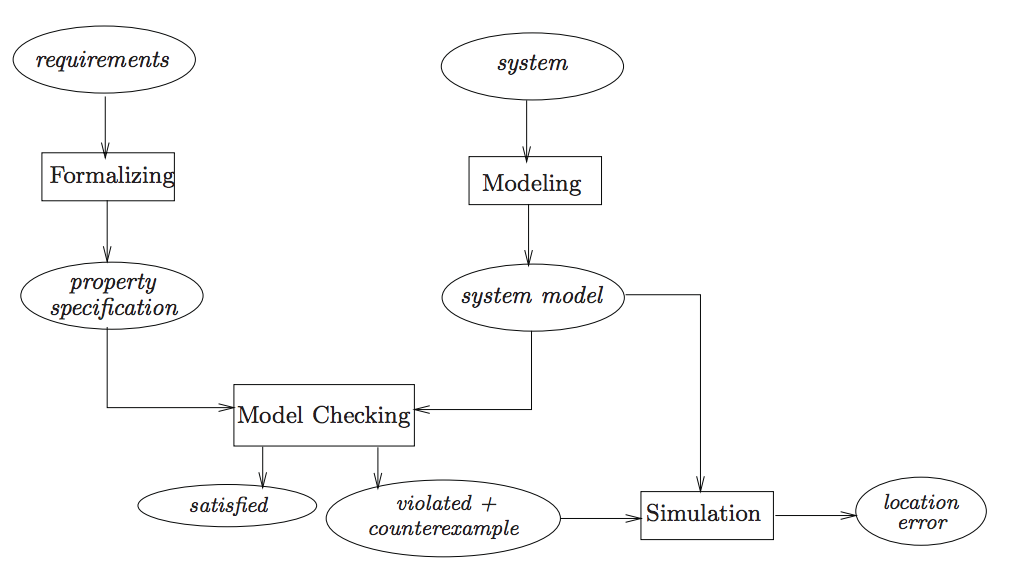
\includegraphics[scale=0.7]{figures/schematic-view.png}
   \caption[Caption for LOF]{Vue schématique de l'approche du model-checking\protect\footnotemark}
   \label{fig:schematic-view}
\end{figure}

\footnotetext{Source: Christel Baier and Joost-Pieter Katoen, Principles of Model Checking \cite{RefBook}, p.8 figure 1.4}

\subsection{Avantages \& désavantages}

Dans cette section, plusieurs avantages et inconvénients seront présentés sur base des recherches effectuées en 2008 par \textit{Clarke} \cite{Birth-MC} ainsi que du livre de référence "Principles of Model Checking" \cite{RefBook}.

\subsubsection{Avantages du model-checking}

Un model-checking possède plusieurs avantages par rapport à l'utilisation d'éventuelles autres techniques de vérifications et de détection d'erreur. Voici une liste non exhaustive de ces avantages : 

\begin{itemize}
\item Il s'agit d'une approche générale de vérification applicable dans tous les domaines tels que les systèmes embarqués ou ingénierie logicielle. 
\item La phase de vérification est automatique. Suivant la phase de modélisation, la seule action nécessaire de l'utilisateur afin de faire fonctionner le model-checking est de l'activer. Le programme s'occupe du reste. Niveau performance, cet automatisme permet un gain de temps conséquent. 
\item Contrairement aux simples tests, le model-checking va également prouver la bonne fonctionnalité du système et dans le cas contraire, nous renvoyer un contre-exemple d'une exécution du système qui falsifie la propriété et ainsi, détecter le(s) bug(s). Le taux d'erreurs non repérés est donc moindre par rapport aux tests simples. 
\item Le model-checking agit sur tout le système et non qu'une seule partie, il s'agit donc d'une méthode exhaustive. Néanmoins, si l'utilisateur le souhaite, il est tout de même possible d'utiliser le model-checking pour une vérification partielle et ainsi l'appliquer à des parties de système. 
\item Utilisation de la logique temporelle (\textit{cfr. \autoref{sec:log-temp} "Introduction à la logique temporelle"}) qui permet d'exprimer facilement les diverses propriétés de manière non ambigüe et universelle. 
\end{itemize}

\subsubsection{Désavantages du model-checking} \label{sec:desavantages}

Néanmoins, le model-checking est une solution discutable sur certains points : 

\begin{itemize}
\item Le model-checking grandit exponentiellement au nombre de processus actifs (appelés états, correspondant à la taille du système). Pour $N$ variables avec un domaine de $k$ valeurs possibles, le nombre d'états grandit de $k^{N}$. Par exemple, pour 20 variables booléennes, il y aurait déjà $2^{20}$ soit 1048576 états. Le modèle devient donc très vite surchargé et surpasse la capacité de la mémoire. Ce problème est appelé \textit{State explosion problem} \cite{StateExpProb}. Par conséquent, le model-checking ne pourrait donc pas croître. Cependant, plusieurs recherches \footnote{La section 5 "State Explosion Problem" de l'article de Clarke \cite{StateExpProb} reprend les principales recherches de solutions à ce problème.} ont été établies dans le but d'établir une solution à ce problème tels que les \textit{diagrammes de décisions binaires} permettant de représenter plusieurs états en un diagramme. 
\item Le model-checking s'applique généralement sur des systèmes finis et n'est pas adapté aux systèmes non-finis de part sa modélisation grâce à des automates d'états finis. Hors, la possibilité de tomber sur un système non-fini (ayant donc une infinité de valeurs possibles pour les variables) n'est pas écartée. % EXPLIQUER PLUS
\item Comme son nom l'indique, le model-checking exécute une vérification du modèle du système et non du système en lui-même. Les résultats obtenus pour le modèle correspondent en grande partie au système réel, néanmoins, il est nécessaire d'utiliser des techniques supplémentaires comme des tests pour trouver les éléments qui pourraient différer entre le modèle et le système réel, que ce soit au niveau du hardware tel que des défauts de fabrication ou bien au niveau software tel que des erreurs de codage. 
\item Conséquence du dernier point : le résultat n'est donc pas garanti à 100\% et pourrait donc contenir des erreurs. 
\end{itemize}

\section{Point de vue algorithmique} \label{sec:pdv-algo}

\subsection{Graphes et principes d'états}
%Présentation du principe de systèmes d'états finis et de graphes en quelques mots + Schéma 
Le model-checking base sa représentation sur un système de graphe orienté, plus précisément sur un \textit{système d'états finis} où chaque noeud du graphe est appelé état tel que les arcs entre ces états sont appelés transitions. Cet ensemble d'états et de transitions décrit le comportement du système réactif et forme le \textbf{modèle} de ce système. \\

Dans l'exemple du problème de distributeur de boissons abordé précédemment, un tel modèle se présenterait comme tel : 

\begin{figure}
  \centering
   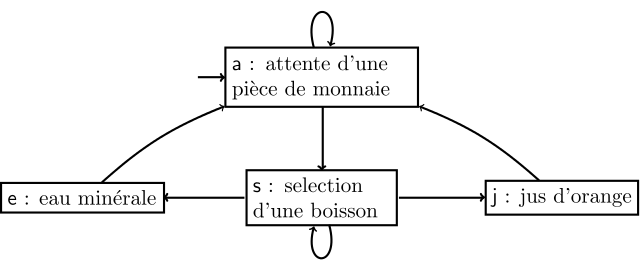
\includegraphics[scale=0.5]{figures/model-boissons.png}
   \caption[Caption for LOF]{Modèle du problème d'un distributeur de boissons\protect\footnotemark}
   \label{fig:model_boissons_1}
\end{figure}

\footnotetext{Source: Wikipedia, "Vérifications de modèles"}

\noindent
où chaque état est définie par un nom (un alias). Par exemple, "a" définit l'attente de l'entrée d'une pièce de monnaie dans la machine. \\

Un modèle de ce type suit la \textbf{structure de Kripke} et est donc appelé \textit{modèle de Kripke}. 

\newpage 

\subsection{Structure de Kripke} \label{sec:kripke}
%Présentation de la structure de Kripke, définitions des différentes notions.

\subsubsection{Définition} 

\textit{Kripke} définit sa structure, donnant nom à la structure de Kripke \cite{Kripke} : 

$$\boxed{\mathcal{K} = (S,I,A,AP,\delta,\lambda)}$$ 


\noindent
tel que : 
\begin{itemize}
\item \textbf{S} est un ensemble fini d'états, \\
\item \boldmath$I \subseteq S$ est l'ensemble des états initiaux, \\
\item \textbf{A} est un ensemble d'actions, \\
\item \textbf{AP} est un ensemble de propositions atomiques, \\
\item \boldmath$\delta \subseteq S \times A \times S$ est une relation de transitions entre états, \\
\item \boldmath$\lambda : S \rightarrow 2^{AP}$ est une fonction de labelisation (étiquetage) des états qui fait correspondre chaque état avec la proposition qui y est liée.  
\end{itemize}

\subsubsection{Exemple complet d'une structure de Kripke} 

Toujours sur base du même problème de distribiteur de boissons, le modèle de la \autoref{fig:model_boissons_1} peut-être repris et complété en se voyant attribuer des noms d'actions afin de pouvoir spécifier les transitions et par conséquent de respecter la structure de Kripke. 

\begin{figure}
  \centering
   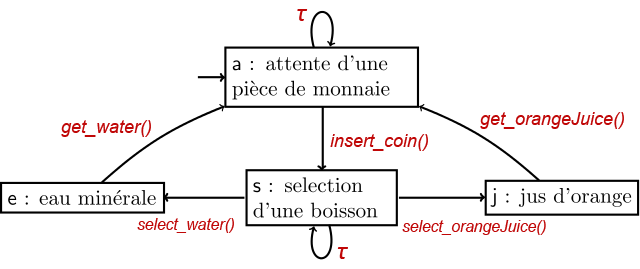
\includegraphics[scale=0.5]{figures/model-boissons-2.png}
   \caption[Caption for LOF]{Modèle de Kripke complet du problème d'un distributeur de boissons}
   \label{fig:model_boissons_2}
\end{figure}

\noindent
Dans ce cas, l'ensemble des états est $S = \{a, e, s, j\}$. L'ensemble des états initiaux $I = \{a\}$ ici ne comporte qu'un seul état initial et est représenté dans le modèle par un arc d'entrée vers l'état initial $a$. \\

\noindent
Les labels associés à chaque transition correspond à une action et fait donc partie de l'ensemble d'action $A$. Le symbole $\tau$ représente une action qui n'est pas particulièrement intéressant à étiquetter mais qui n'est néanmoins pas à négliger tels que l'attente de la pièce ou une non-sélection de boisson. L'ensemble d'action est donc $A = \{select\_water, select\_orangeJuice, insert\_coin, get\_orangeJuice, \tau\}$. \\

\noindent
Les états et actions maintenant définies, des exemples de relations de transitions peuvent être présentés. Voici les transitions d'états lors de l'achat d'un jus d'orange dans le distributeur : 

\begin{enumerate}
\item \boldmath$\delta(a,insert\_coin,s)$ : représente la transition de l'état \textit{attente d'une pièce de monnaie} à l'état \textit{sélection d'une boisson} grâce à l'action d'insertion de pièce \textit{insert\_coin}. 
\item \boldmath$\delta(s,select\_orangeJuice,j)$ : représente la transition de l'état \textit{sélection d'une boisson} à l'état \textit{jus d'orange} grâce à l'action \textit{select\_orangeJuice}. 
\item \boldmath$\delta(j,get\_orangeJuice,a)$ : représente la transition de l'état \textit{jus d'orange} à l'état \textit{attente d'une pièce de monnaie} grâce à l'action \textit{get\_orangeJuice}.
\end{enumerate} 

Ces 3 exemples de transitions font partie des 7 transitions d'états possibles du modèle. \\

\noindent
Finalement, concernant le choix des propositions atomiques, le choix le plus simple est d'utiliser le nom des états comme propositions atomiques.\\
La fonction de labelisation serait donc $\lambda(s) = \{s\}  \forall s \in S$.  

\subsection{Arbre d'exécution d'une structure de Kripke}

\subsubsection{Définition} 
Un \textit{arbre d'exécution d'une struture de Kripke} correspond au "dépliage" du modèle de Kripke où les noeuds correspondent aux états tel que la racine est l'état initial du modèle de Kripke. Au niveau i, les fils d'un noeud sont les états successeurs au niveau i+1, c'est-à-dire les états subissant une transition à partir du noeud du niveau i. 

\subsubsection{Pourquoi utiliser un arbre ?}
L'utilisation d'un arbre permet de représenter tous les chemins de la structure de Kripke. Lorsque le graphe de Kripke est cyclique, l'arbre résultant est un arbre infini. C'est notamment de cette transformation en arbre que le model checking CTL (Computation Tree Logic) tient son nom vu qu'il se base sur la structure en arbre du système. 

\subsubsection{Illustration : d'un graphe à un arbre.}

Afin d'illustrer la transformation de la structure de Kripke à un arbre, reprenons une nouvelle fois l'exemple du distributeur de boissons dont le modèle de Kripke est présentée à la \autoref{fig:model_boissons_2} et transformons celui-ci en arbre. 

\begin{figure}
  \centering
   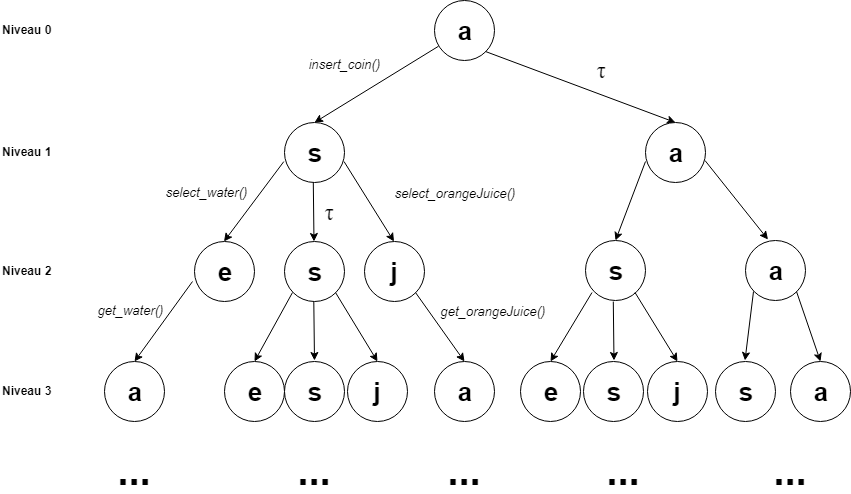
\includegraphics[scale=0.5]{figures/Arbre_Distributeur.png}
   \caption[Caption for LOF]{Arbre du problème d'un distributeur de boissons}
   \label{fig:arbre_boissons}
\end{figure}

Tous les éléments présents dans le modèle de Kripke se retrouvent bien dans l'arbre. Dans ce cas, il s'agit bien d'un arbre infini résultant d'un graphe cyclique dont les 4 premiers niveaux sont présentés dans la \autoref{fig:arbre_boissons}. Le niveau 0 représente la racine de l'arbre et donc l'état initial du système. 

 
\section{Le model-checking de CTL: généralités et logiques}

\subsection{Introduction à la logique temporelle} \label{sec:log-temp}
%Première approche de la notion de logique temporelle, des différentes sortes de logiques temporelles existantes (linéaire ou arborescente), des propositions de logiques temporelles, des formules associés, ... 
Les différentes propriétés du système à vérifier sont exprimés via la notion de \textit{logique temporelle}. Celle-ci forme le deuxième élément complémentaire aux systèmes d'états finis (modèle de Kripke) permettant la réalisation de l'étape de modélisation du model checking. 

La logique temporelle définit les propriétés temporelles à l’aide de connecteurs temporels\footnote{N.B: Il s'agit bien d'une logique temporelle et non temporisée, cette logique ne quantifie donc pas l'écoulement du temps mais décrit bien l'ordre des événements sans introduire la notion de temps explicitement.} ("until", "next", "always", ...) et de quantificateurs sur les états ou les chemins de son graphe. Cette logique permet donc d'exprimer et vérifier des propriété de sûreté (absence de bugs), d’absence de blocages de l’exécution, d'invariance (tous les états satisfont une propriété) ou d'équité (fonctionnel et répétable infiniment) et remplit donc parfaitement le rôle de vérification du model checking. \\

Les deux principaux types de logiques temporelles qui seront abordés prochainement sont \textbf{la logique temporelle linéaire} (LTL) et \textbf{la logique temporelle arborescente} (CTL). Cependant, il existe également d'autres types de logiques temporelles tels que CTL* (fusion entre LTL et CTL), mucalcul, ForSpec, PSL, \dots 

\subsection{Un premier aperçu de LTL et CTL}

\subsubsection{Linear Temporal Logic - LTL}
La logique temporelle linéaire ne quantifie pas sur les états et considère donc seulement des traces linéaires. Elle étend la logique classique par des modalités temporelles présentés dans la \autoref{fig:operateurs-temp} qui référence vers différents moments dans le temps (passé ou futur). 

\begin{figure}
  \centering
   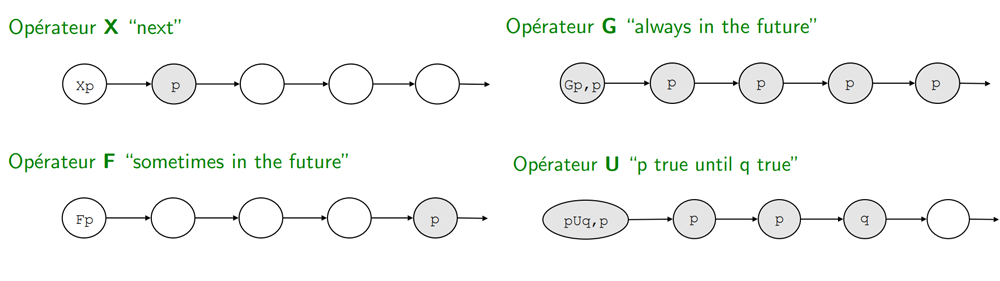
\includegraphics[scale=0.43]{figures/operateurs-temp.png}
   \caption[Caption for LOF]{Modalités temporelles de LTL\protect\footnotemark}
   \label{fig:operateurs-temp}
\end{figure}

\footnotetext{Source: Sébastien Bardin http://sebastien.bardin.free.fr/MC-cours2.pdf - Slides 7/44} 

\subsubsection{Computation Tree Logic - CTL}
CTL est une logique temporelle basée sur la logique propositionnelle avec une notion discrète du temps dont le future n'est pas déterminé. CTL offre notamment une logique temporelle en arbre permettant la formulation d'un ensemble conséquent de propriétés. En effet, CTL exprime tous les chemins possibles d'un état à un autre grâce à sa structure d'arbre (notamment les arbres résultant du modèle de Kripke). En d'autres termes, la logique temporelle arborescente CTL peut être définie à partir d’un ensemble de variables propositionnelles AP, des connecteurs classiques de la logique propositionnelle tels que l'implication, la conjonction ou la disjonction, de quantificateurs de chemins (E ou A) et de connecteurs temporels (X,F,G,U). La syntaxe et sémantique de CTL fera l'objet des \autoref{sec:syntaxe-CTL} et \autoref{sec:sem-CTL}. \\

\subsection{Syntaxe de CTL} \label{sec:syntaxe-CTL}
Comme expliqué ci-dessus, la logique temporelle arborescente CTL est basée sur la logique propositionnelle et définit donc chaque connecteur de cette logique ainsi que d'autres connecteurs temporels propres à CTL. Cet ensemble forme la syntaxe de la logique temporelle arborescente CTL et est présentée comme tel : \\

Soit: \\
$\mathbb{V}$ un ensemble dénombrable de variables propositionnelles, \\
$C$ un ensemble fini de connecteurs propositionnels: $C = \{\wedge, \vee, \neg, \Rightarrow, \Leftrightarrow \}$, \\
$T$ un ensemble fini de connecteurs temporels : $T = \{X, F, G, U, A, E\}$ \\

Tel que:\\
$\mathbb{V} \subseteq CTL$ (variables propositionnelles sont donc des formules CTL), \\
$\phi$, $\phi_{1}, \phi_{2}$ des propriétés quelconques $\in CTL$ \\

Alors: \\

\begin{center}
\begin{tabular}{|c|c|c|}
  \hline
  Syntaxe & Notation française & Signification \\
  \hline
  $\neg\phi_{1}$ & NON $\phi_{1}$ & Négation de $\phi_{1}$ \\
  $\phi_{1} \wedge \phi_{2}$ & $\phi_{1}$ ET $\phi_{2}$ & Conjonction de $\phi_{1}$ et $\phi_{2}$\\
  $\phi_{1} \vee \phi_{2}$ & $\phi_{1}$ OU $\phi_{2}$ & Disjonction de $\phi_{1}$ et $\phi_{2}$\\
  $\phi_{1} \Rightarrow \phi_{2}$ & $\phi_{1}$ IMPLIQUE $\phi_{2}$ & Implication de $\phi_{1}$ vers $\phi_{2}$\\
  $\phi_{1} \Leftrightarrow \phi_{2}$ & $\phi_{1}$ EQUIVAUT $\phi_{2}$ & Double implication (équivalence) de $\phi_{1}$ et $\phi_{2}$\\
 \hline
 
\end{tabular}
\captionof{table}{Syntaxe de CTL - Logique propositionnelle} \label{tab:syntax-ctl-prop}
\end{center}

\begin{center}
\begin{tabular}{|c|c|c|}
  \hline
  Syntaxe & Signification \\
  \hline
  $AX\phi$ & Dans tous les chemins ($A$), $\phi$ est valide pour le prochain état du chemin. ($X$)\\
  $AF\phi$ & Dans tous les chemins ($A$), $\phi$ est valide pour au moins un état du chemin. ($F$) \\
  $AG\phi$ & Dans tous les chemins ($A$), $\phi$ est valide pour tous les états du chemin. ($G$) \\
  $A(\phi_{1} \cup \phi_{2})$ & Dans tous les chemins ($A$), $\phi_{1}$ est valide jusqu'à ce que $\phi_{2}$ devient valide ($\cup$) \\
  \hline
  $EX\phi$ & Il existe un chemin ($E$) où $\phi$ est valide pour le prochain état du chemin. ($X$) \\
  $EF\phi$ & Il existe un chemin ($E$) où $\phi$ est valide pour au moins un état du chemin. ($F$)\\
  $EG\phi$ & Il existe un chemin ($E$) où $\phi$ est valide pour tous les états du chemin. ($G$)\\
  $E(\phi_{1} \cup \phi_{2})$ & Il existe un chemin ($E$) où $\phi_{1}$ est valide jusqu'à ce que $\phi_{2}$ devient valide ($\cup$) \\
  
 \hline
 
\end{tabular}
\captionof{table}{Syntaxe de CTL - Logique temporelle} \label{tab:syntax-ctl-temp}
\end{center}

La \autoref{tab:syntax-ctl-prop} reprend les connecteurs principaux de la logique propositionnelle tandis que la \autoref{tab:syntax-ctl-temp} correspondant à de la logique temporelle. Cette dernière est divisée selon les quantificateurs de chemins en deux parties : 
\begin{itemize}
\item \textbf{A} pour "\textbf{A}ll" : la propriété est valide sur tous les chemins possibles (= inévitable).
\item \textbf{E} pour "\textbf{E}xists" : la propriété est valide sur minimum un chemin (= possible).
\end{itemize}

Chacune de ses parties possède 4 types de connecteurs : 
\begin{itemize}
\item \textbf{X} pour "ne\textbf{X}t" : la propriété doit être valide pour le prochain état du chemin. 
\item \textbf{F} pour "\textbf{F}inally" : la propriété est valide pour au moins un état du chemin.
\item \textbf{G} pour "\textbf{G}lobally" : la propriété est valide pour tous les états du chemin.
\item $\pmb{\cup}$ pour "\textbf{U}ntil" : la propriété doit être valide jusqu'à ce que la deuxième est "déclenchée" et devient donc valide. \\
\end{itemize}

La logique temporelle présentée à la \autoref{tab:syntax-ctl-temp} est illustrée dans la \autoref{fig:syntax-schema}. 

\begin{figure}
  \centering
   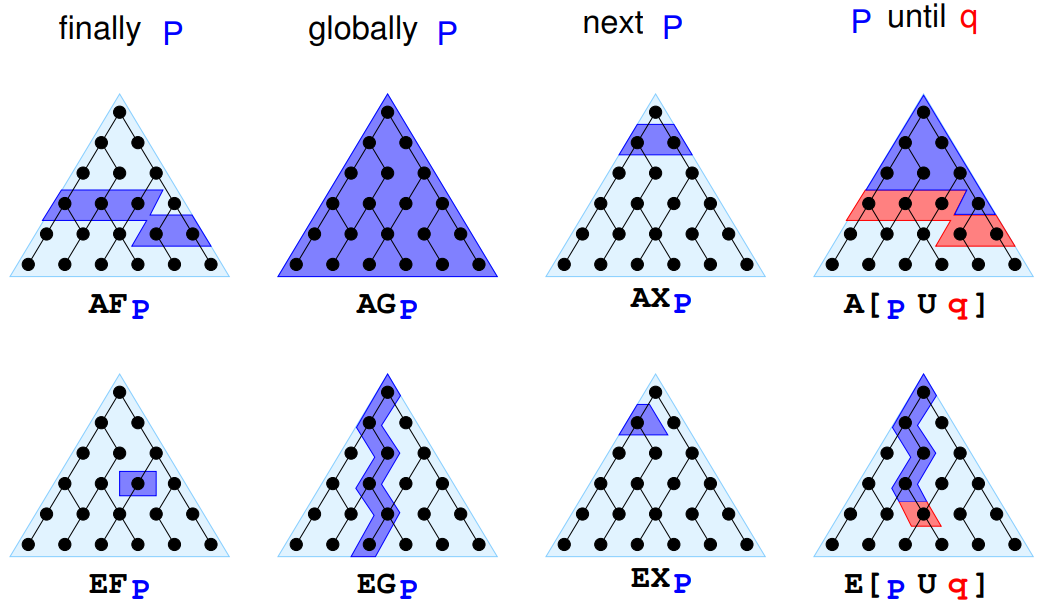
\includegraphics[scale=0.43]{figures/syntax-schema.png}
   \caption[Caption for LOF]{Illustration de la logique temporelle de CTL\protect\footnotemark}
   \label{fig:syntax-schema}
\end{figure}

\footnotetext{Source: Alessandro Artale (2010) http://www.inf.unibz.it/~artale/FM/slide4.pdf - Slide 14/37} 


% AJOUTER PROPRIETES SI BCP DE PAGES ACCEPTE  (http://www.inf.ed.ac.uk/teaching/courses/propm/papers/CTL.pdf slide 10 + https://www.cs.cmu.edu/~emc/15414-s14/lecture/ModelChecking.pdf slide 17) et EXEMPLE DISTRI avec SYNTAXE


\newpage
\subsection{Sémantique de CTL} \label{sec:sem-CTL}
%Présentation de la sémantique de CTL - des relations de satisfactions, des interprétations des différentes formules, etc.. 
Les formules CTL sont interprétées par rapport aux états et aux chemins d'un système de transisition (qui suit la structure de Kripke\footnote{cfr. \autoref{sec:kripke}}). Généralement, la sémantique de CTL aborde donc une formule CTL (propriété) $\phi$ par deux relations de satisfactions, une pour les états $s$ et l'autre pour les chemins $\pi$ :

\begin{enumerate}
\item Pour un état :  $(\mathcal{K},s) \vDash \phi \Leftrightarrow s$ satisfait $\phi$ 
\item Pour un chemin : $(\mathcal{K},\pi) \vDash \phi \Leftrightarrow \pi$ satisfait $\phi$ 
\end{enumerate}

où $\mathcal{K} = (S,I,A,AP,\delta,\lambda)$ est une structure de Kripke.\\

Ces relations de satisfactions sont notamment définies par la logique propositionnelle : 

\begin{center}
\begin{tabular}{lll}
   $(\mathcal{K},s) \vDash \neg\phi$ & \hspace{0.5cm} $\Leftrightarrow$ \hspace{0.5cm} & $\neg s \vDash \phi$  \\
   $(\mathcal{K},s) \vDash \phi_{1} \wedge \phi_{2} $ & \hspace{0.5cm} $\Leftrightarrow$ \hspace{0.5cm} & $(s \vDash \phi_{1}) \wedge (s \vDash \phi_{2})$ \\
   $(\mathcal{K},s) \vDash \phi_{1} \vee \phi_{2} $ & \hspace{0.5cm} $\Leftrightarrow$ \hspace{0.5cm} & $(s \vDash \phi_{1}) \vee (s \vDash \phi_{2})$ \\
   $(\mathcal{K},s) \vDash \exists\phi$ & \hspace{0.5cm} $\Leftrightarrow$ \hspace{0.5cm} & $\pi \vDash \phi$ pour minimum un chemin $\pi \in$ Chemins(s) \\ 
   $(\mathcal{K},s) \vDash \forall\phi$ & \hspace{0.5cm} $\Leftrightarrow$ \hspace{0.5cm} & $\pi \vDash \phi$ pour tous les chemins $\pi \in$ Chemins(s) \\ 
\end{tabular}
\end{center}

De plus, pour vérifier la satisfaction d'une propriété $\phi$ d'une structure de Kripke $\mathcal{K}$ , la logique temporelle caractérise également la sémantique :

 
\begin{center}
\begin{tabular}{lll}
   $(\mathcal{K},s) \vDash AX\phi$ & \hspace{0.5cm} $\Leftrightarrow$ \hspace{0.5cm} & $\forall s'$ tel que $(s,s')\in \delta$ : $s' \vDash \phi$  \\
   $(\mathcal{K},s) \vDash AF\phi$ & \hspace{0.5cm} $\Leftrightarrow$ \hspace{0.5cm} & $\forall \pi \exists i\ge 0$ tel que $\pi_{i} \vDash \phi$  \\
   $(\mathcal{K},s) \vDash AG\phi$ & \hspace{0.5cm} $\Leftrightarrow$ \hspace{0.5cm} & $\forall \pi \forall i\ge 0$ : $\pi_{i} \vDash \phi$  \\
   $(\mathcal{K},s) \vDash A(\phi_{1} \cup \phi_{2})$ & \hspace{0.5cm} $\Leftrightarrow$ \hspace{0.5cm} & $(\forall \pi \exists i\ge 0$ tel que $\pi_{i} \vDash \phi_{2}) \wedge (\forall j \in 0 \le j < i$ : $\pi_{j} \vDash \phi_{1})$ \\
   $(\mathcal{K},s) \vDash EX\phi$ & \hspace{0.5cm} $\Leftrightarrow$ \hspace{0.5cm} & $\exists s'$ tel que $(s,s')\in \delta \wedge (s' \vDash \phi)$  \\
   $(\mathcal{K},s) \vDash EF\phi$ & \hspace{0.5cm} $\Leftrightarrow$ \hspace{0.5cm} & $\exists \pi$ tel que $\exists i \ge 0$ tel que $\pi_{i} \vDash \phi$  \\
   $(\mathcal{K},s) \vDash EG\phi$ & \hspace{0.5cm} $\Leftrightarrow$ \hspace{0.5cm} & $\exists \pi$ tel que $\forall i\ge 0$ : $\pi_{i} \vDash \phi$  \\
   $(\mathcal{K},s) \vDash E(\phi_{1} \cup \phi_{2})$ & \hspace{0.5cm} $\Leftrightarrow$ \hspace{0.5cm} & $(\exists \pi$ tel que $\exists i \ge 0$ tel que $\pi_{i} \vDash \phi_{2}) \wedge (\forall j \in 0 \le j < i$ : $\pi_{j} \vDash \phi_{1})$ \\
\end{tabular}
\end{center}

\subsubsection{Equivalence sémantique} 

Deux formules CTL $\phi_{1}$ et $\phi_{2}$ sont équivalents, dénoté $\phi_{1} \equiv \phi_{2}$, lorsqu'ils sont sémantiquements identiques, c'est-à-dire que pour chaque état $s$ : $s \vDash \phi_{1} \Leftrightarrow s \vDash \phi_{2}$.

\newpage

\textbf{Exemples d'équivalence sémantique} \\ 

\begin{itemize}
\item Les lois de De Morgan formulés en CTL : \\

\begin{center}
$\neg AF\phi \equiv EG\neg\phi$ \\
$\neg EF\phi \equiv AG\neg\phi$ \\
$\neg AX\phi \equiv EX\neg\phi$ \\
\end{center}

\item Les lois d'expansions : \\

\begin{center}
$ AG\phi \equiv \phi \wedge AXAG\phi$ \\
$ EG\phi \equiv \phi \wedge EXEG\phi$ \\
$ AF\phi \equiv \phi \vee AXAF\phi$ \\
$ EF\phi \equiv \phi \vee EXEF\phi$ \\
$ A(\phi_{1}\cup\phi_{2}) \equiv \phi_{2} \vee (\phi_{1} \wedge AXA(\phi_{1}\cup\phi_{2})$ \\
$ E(\phi_{1}\cup\phi_{2}) \equiv \phi_{2} \vee (\phi_{1} \wedge EXE(\phi_{1}\cup\phi_{2})$ \\
\end{center}

\end{itemize}


\subsubsection{Sûreté et vivacité d'un système}

Deux définitions importantes concernant le bon fonctionnement d'un système peuvent maintenant être exprimées : 

\begin{enumerate}
\item Un système est dit \textbf{sûr} lorsqu'il est garanti que quelque chose de "mauvais" ne va jamais se produire et peut être exprimer par la formule CTL $AG\neg bad$.  Si ce n'est pas le cas alors il existe un nombre fini de contre-exemples. 
\item Un système est dit \textbf{vivant} lorsqu'il est garanti que quelque chose de "bon" va toujours se produire et peut être exprimer par la formule CTL $AGAFgood$. Si ce n'est pas le cas alors il existe un nombre fini de contre-exemples. 
\end{enumerate}



\subsection{Comparaison LTL/CTL}

\subsubsection{Caractéristiques générales}
\begin{itemize}
\item LTL est limité à une représentation linéaire du système mais ses connecteurs temporels permettent d'exprimer le futur ainsi que le passé. 
\item CTL offre une représentation complète en arbre présentant tous les chemins possibles et donc une grand nombre de propriétés potentiels exprimés, ce qui fait donc de lui un model-checking efficace. Néanmoins, les connecteurs temporels utilisés ne permettent d'exprimer uniquement le temps futur. 
\end{itemize} 


\subsubsection{Expressivité}
\begin{itemize}
\item LTL décrit les propriétés d'une exécution à la fois. LTL est donc très expressif sur un chemin mais il n'y a aucune expressivité sur les futures possibles. 
\item CTL raisonne sur un comportement arborescent en considérant plusieurs exécutions possible en même temps. CTL pourrait donc manquer d'expressivité linéaire mais est très expressif concernant les futures potentiels. \\
\end{itemize}

De ce fait, certaines propriétés CTL (LTL) ne sont pas expressibles en LTL (CTL) ou est considéré d'une autre façon d'une logique à une autre. Pour citer des exemples : 

\begin{itemize}
 \renewcommand{\labelitemi}{\scriptsize$\bullet$}
 \item  $AGEF\phi$ (appelé \textit{"reset property"}) est une formule CTL qui n'est pas expressible en LTL.
 \item La formule CTL $AFAXp$ distingue les deux systèmes présentés dans la \autoref{fig:CTL-EXPR-2} tandis que la formule LTL $FXp$ ne le distingue pas. 
 
 \begin{figure}
  \centering
   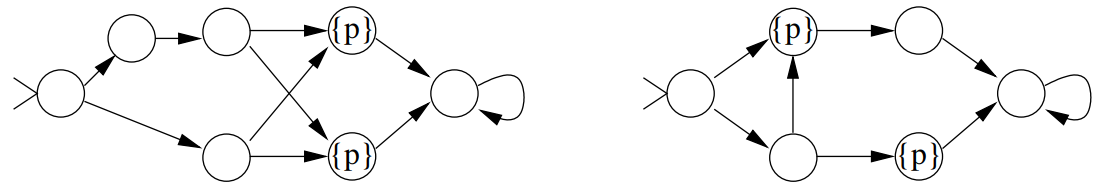
\includegraphics[scale=0.43]{figures/CTL-EXPR-2.png}
   \caption[Caption for LOF]{Exemple 2 - Expressivité CTL/LTL}
   \label{fig:CTL-EXPR-2}
\end{figure}

\item La formule LTL $FGp$ n'est pas expressible en CTL comme illustré dans la \autoref{fig:CTL-EXPR-3}. \\

 \begin{figure}
  \centering
   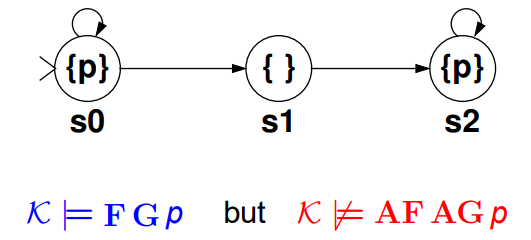
\includegraphics[scale=0.43]{figures/CTL-EXPR-3.png}
   \caption[Caption for LOF]{Exemple 3 - Expressivité CTL/LTL}
   \label{fig:CTL-EXPR-3}
\end{figure}

\end{itemize}

L'utilisation des deux types de logiques temporelles LTL et CTL est donc nécessaire ; l'expressivité de ces deux logiques n'est pas comparable, elles sont complémentaires : chaque logique possède des propriétés que l'autre ne peut pas exprimer. 



\newpage
\subsubsection{Complexité théorique}
\begin{itemize}
\item La complexité d'un problème de model checking utilisant LTL est PSPACE-complet. Plus particulièrement, sa complexité est en $\mathcal{O}(|TS| \cdot exp(|\phi|))$ où $|TS|$ correspond à la taille du système de transition et $|\phi|$ la taille de la propriété à vérifier. 
\item La complexité d'un problème de model checking utilisant CTL est PTIME. Plus particulièrement, sa complexité est en $\mathcal{O}(|TS| \cdot |\phi|)$ où $|TS|$ correspond à la taille du système de transition et $|\phi|$ la taille de la propriété à vérifier. 
\end{itemize}


\subsubsection{En pratique}
\begin{itemize}
\item LTL (étendu avec des expressions régulières) est généralement utilisé dans l'industrie des processeurs. Il est notamment très intuitif au niveau des contres-exemples et de l'interface et permet la vérification au run-time par tests. LTL vérifie donc des propriétés compliquées mais uniquement sur des parties de système. 
\item CTL est utilisé pour une vérification de propriétés simples sur un système entier et donc en d'autres termes, effectue une vérification du modèle. 
\end{itemize}




\section{Le model-checking CTL: algorithme et implémentation}
\subsection{Pseudo-code de l'algorithme}
Pseudo-code (ou code personnel) simple d'un algorithme de Model Checking CTL.
% pseudo code basé sur des implémentations  

\subsection{Analyses et résultats}
Analyse détaillée du code de l'algorithme et présentation résultats obtenus 

\subsection{Complexité}
Complexité du code donné ainsi que d'un model checking de CTL en général \\ 


\bibliographystyle{unsrt}
\nocite{*}
\bibliography{bibliography}


\end{document}
